%写在前面:
%建议首先阅读 README.txt
%本模版是【非官方】中央财经大学课程论文模版。因为使用本模版造成任何问题由使用者【自行承担】。

%注意:使用时,请使用XeLaTeX进行编译,不要用overleaf默认的pdfLaTeX进行编译。

%关于产权:
%本模版改编自:DoniaHakurei在GitHub的仓库中上传的模版(https://github.com/DoniaHakurei/CUFE_thesis_LaTeX_template)。原模版在某些地方,如封面的字体等不符合教务处最新要求,因此本人进行了相应修改。
%同时,本模版已经上传在本人的个人GitHub仓库中(个人主页:https://github.com/NathanHuXy)。
%作者:胡雪岩(金融科技20)
%邮箱:1033739554@qq.com

%请尊重作者产权。


%---------------------------------------------------------------------
%	个性化信息
%--------------------------------------------------------------------
\newcommand{\MYTITLE}{非银企业的债券期限结构是否合理}%论文标题
\newcommand{\MYNAME}{代旭科 2022310417}%姓名
\newcommand{\MYCLASS}{金融科技22}%班级
\newcommand{\MYADVISOR}{杜涣程}%任课教师
\newcommand{\MYCOURSE}{金融统计分析}%课程名
\newcommand{\MYTERM}{2024-2025 第一学期}%学期


%---------------------------------------------------------------------
%   各种导言
%--------------------------------------------------------------------
\documentclass[a4paper,12pt]{report}
\usepackage{geometry} % to change the page dimensions
\geometry{a4paper,left=2.5cm,right=2.5cm,top=2.54cm,bottom=2.54cm}%页边距
\usepackage{ctex}
\usepackage{xeCJK}
\usepackage{comment}
\usepackage{setspace}
\usepackage{fancyhdr}
\usepackage{graphicx}
\usepackage{wrapfig}
\usepackage{subfigure}
\usepackage{array}
\usepackage{titlesec}
\usepackage{titletoc}
\usepackage[titletoc]{appendix}
%\usepackage[top=30mm,bottom=30mm,left=20mm,right=20mm]{geometry}
%\usepackage{cite}

\setstretch{1.5}
%\usepackage{courier}
\setmonofont{Courier New}
\usepackage{listings}
%---------------------------------------------------------------------
%   参考文献设置
%--------------------------------------------------------------------
\usepackage[backend = biber, style = references/gb7714-2015, defernumbers=true]{biblatex}
\renewcommand*{\bibfont}{\small}
\addbibresource{references/bibs.bib}
\renewcommand{\bibname}{参考文献}
%---------------------------------------------------------------------
%	引用文献设置为上标
%---------------------------------------------------------------------
\begin{comment}
    \makeatletter
    \def\@cite#1#2{\textsuperscript{[{#1\if@tempswa , #2\fi}]}}
    \makeatother
\end{comment}

\lstset{tabsize=4, keepspaces=true,
    xleftmargin=2em,xrightmargin=0em, aboveskip=0.1em,
    %backgroundcolor=\color{gray!20},  % 定义背景颜色
    frame=none,                       % 表示不要边框
    extendedchars=false,              % 解决代码跨页时,章节标题,页眉等汉字不显示的问题
    numberstyle=\ttfamily,
    basicstyle=\ttfamily,
    keywordstyle=\color{blue}\bfseries,
    breakindent=10pt,
    identifierstyle=,                 % nothing happens
    commentstyle=\color{green}\small,  % 注释的设置
    morecomment=[l][\color{green}]{\#},
    numbers=left,stepnumber=1,numberstyle=\scriptsize,
    showstringspaces=false,
    showspaces=false,
    flexiblecolumns=true,
    breaklines=true, breakautoindent=true,breakindent=4em,
    escapeinside={/*@}{@*/},
}
\usepackage{amsmath}
\usepackage{amsthm}
\newtheorem{theorem}{定理}
\newtheorem{definition}{定义}
\newtheorem{corollary}{推论}
\newtheorem{example}{例}
\renewcommand {\thetable} {\arabic{table}}
\renewcommand {\thefigure} {\arabic{figure}}
\usepackage{amsfonts}
\usepackage{lipsum}
%\usepackage{bm}
\usepackage{booktabs} % for much better looking tables
\usepackage{paralist} % very flexible & customisable lists (eg. enumerate/itemize, etc.)
\usepackage{verbatim} % adds environment for commenting out blocks of text & for better verbatim
\usepackage{subfigure} % make it possible to include more than one captioned figure/table in a single float
% These packages are all incorporated in the memoir class to one degree or another...
\usepackage{cases} %equation set
\usepackage{multirow} %use table
\usepackage{algorithm}
\usepackage{algorithmic}
%\usepackage{cite}
\usepackage{hyperref}
\usepackage{longtable}
\usepackage{caption}
\usepackage{zhnumber} % change section number to chinese
\usepackage{color}
\hypersetup{colorlinks,linkcolor=black,anchorcolor=black,citecolor=black, pdfstartview=FitH,bookmarksnumbered=true,bookmarksopen=true,} % set href in tex & pdf
%\usepackage[framed,numbered,autolinebreaks,useliterate]{mcode} % 插入matlab代码
\XeTeXlinebreaklocale "zh"
\XeTeXlinebreakskip = 0pt plus 1pt minus 0.1pt
\setlength{\baselineskip}{22pt}
%---------------------------------------------------------------------
%	图表顺序标号,不分章节
%---------------------------------------------------------------------
\usepackage{chngcntr}
\counterwithout{table}{chapter}
\counterwithout{table}{section}
\counterwithout{figure}{chapter}
\counterwithout{figure}{section}
\counterwithout{equation}{chapter}
\counterwithout{equation}{section}


\titleclass{\chapter}{straight}%禁止chapter换页
%---------------------------------------------------------------------
%	页眉页脚设置
%---------------------------------------------------------------------
\fancypagestyle{plain}{
    \pagestyle{fancy}      %改变章节首页页眉
}

\pagestyle{fancy}
\lhead{}
\rhead{}
\fancyhead[C]{\MYTITLE}
\cfoot{\thepage}
\renewcommand\thesection{(\zhnum{section})}
\renewcommand \thesubsection {\arabic{subsection}.}
\renewcommand \thechapter {\zhnum{chapter}、}
\titleformat{\chapter}{\centering\zihao{4}\songti\bfseries}{\chinese{chapter}、}{0.05em}{}
\titlespacing{\chapter}{12pt}{12pt}{*3}
\titlespacing{\section}{0pt}{0pt}{*0}
\titlespacing{\subsection}{0pt}{0pt}{*0}
\titleformat{\section}{\zihao{-4}\songti\bfseries}{$\qquad$(\chinese{section})}{0.05em}{}
\titleformat{\subsection}{\zihao{-4}\songti}{$\qquad$\arabic{subsection}.$\ $}{0.05em}{}

%---------------------------------------------------------------------
%	摘要设置
%---------------------------------------------------------------------
%\renewcommand{\abstractname}{摘要}
\newcommand{\enabstractname}{ABSTRACT}
\newcommand{\cnabstractname}{内\quad 容\quad 摘\quad 要}
\newenvironment{enabstract}{%
  \par\small
  \noindent\mbox{}\hfill{\bfseries \zihao{3} \enabstractname}\hfill\mbox{}\par
  \vskip 2.0ex}{\par\vskip 2.0ex}
\newenvironment{cnabstract}{%
  \par\small
  \noindent\mbox{}\hfill{\bfseries \zihao{3} \cnabstractname}\hfill\mbox{}\par
  \vskip 2.0ex}{\par\vskip 2.0ex}
\renewcommand{\figurename}{图}
\renewcommand{\tablename}{表}
%---------------------------------------------------------------------
%	目录页设置
%---------------------------------------------------------------------
%\renewcommand{\contentsname}{\zihao{-3} 目\quad 录}
\setcounter{tocdepth}{1}
\renewcommand{\contentsname}{\zihao{3}\bfseries\centering{目$\quad$录}}
\titlecontents{chapter}[0em]{\songti\zihao{4}\bfseries}{\thecontentslabel\ }{}
{\hspace{.5em}\titlerule*[4pt]{$\cdot$}\contentspage}
\titlecontents{section}[2em]{\vspace{0.1\baselineskip}\songti\zihao{4}}{\thecontentslabel\ }{}
{\hspace{.5em}\titlerule*[4pt]{$\cdot$}\contentspage}
%\titlecontents{subsection}[4em]{\vspace{0.1\baselineskip}\songti\zihao{-4}}{\thecontentslabel\ }{}
%{\hspace{.5em}\titlerule*[4pt]{$\cdot$}\contentspage}

\begin{document}
%---------------------------------------------------------------------
%	封面设置
%---------------------------------------------------------------------
    \begin{titlepage}
        \begin{center}
            \includegraphics[width=1.0\textwidth]{figure/zhongcai.png}\\
            \vspace{20mm}
            %\textbf{\zihao{2}{\heiti\textbf{\MYTITLE}}}\\[0.8cm]
            \vspace{10mm}
            %\vspace{\fill}

            \setlength{\extrarowheight}{3mm}
            {\kaishu \zihao{4}
                \begin{tabular}{rp{8cm}<{\centering}}
                    {\makebox[4\ccwd][s]{学年学期:}}       & \kaishu \underline{\makebox[8cm]{\MYTERM}}     \\
                    {\makebox[4\ccwd][s]{课程名称:}}       & \kaishu \underline{\makebox[8cm]{\MYCOURSE}}   \\
                    {\makebox[4\ccwd][s]{任课教师:}}       & \kaishu \underline{\makebox[8cm]{\MYADVISOR}}  \\
                    {\makebox[4\ccwd][s]{班\qquad 级:}}    & \kaishu \underline{\makebox[8cm]{\MYCLASS}}    \\
                    {\makebox[4\ccwd][s]{组\qquad 员:}} & \kaishu \parbox[t]{8cm}{\underline{\makebox[8cm]{代旭科 2022310417}}\\
                    \underline{\makebox[8cm]{郭峻荣 2022310408}}\\
                    \underline{\makebox[8cm]{曾子桐 2022310391}}\\
                    \underline{\makebox[8cm]{赵博涵 2022310434}}} \\
                    \\
                \end{tabular}
            }\\[2cm]
        \end{center}
    \end{titlepage}

    %---------------------------------------------------------------------
    %  摘要页
    %---------------------------------------------------------------------
    \setcounter{page}{1}

    \begin{center}
        {\zihao{2} \heiti  \MYTITLE}
    \end{center}
    \vspace{2em}

    \begin{cnabstract}
        本文基于中国非银企业债券市场的发行数据,通过构建不同观察时间窗口和不同观察视角的HHI(赫芬达尔-赫希曼指数)时间序列,
        分析了非银企业债券期限结构的合理性。研究发现,从市场整体层面来看,非银企业债券期限分布较为分散,整体期限结构较为合理且随时间变化不显著;
        但从企业层面观察,单个企业债券期限的集中度较高,存在期限结构不均衡的问题。
        不过,企业层面的债券期限分布呈现逐步改善的趋势,显示了市场机制和政策引导的积极作用。
        本文的研究为进一步优化非银企业债券期限结构、降低期限集中度提供了参考依据。

        \par\textbf{关键词: } 债券,非银企业,期限结构,HHI,市场分布
    \end{cnabstract}


    \begin{enabstract}
        This paper analyzes the rationality of the bond maturity structure of non-financial enterprises in China based on their bond issuance data by constructing HHI (Herfindahl-Hirschman Index) time series with different observation windows and perspectives. The study reveals that, at the market level, the bond maturity structure of non-financial enterprises is relatively dispersed, indicating a reasonable overall structure with insignificant temporal changes. However, at the firm level, individual enterprises exhibit high concentration in bond maturities, highlighting an imbalance in the maturity structure. Nonetheless, the firm-level distribution shows a gradual improvement trend, reflecting the positive impact of market mechanisms and policy guidance. This study provides insights for further optimizing the maturity structure of non-financial enterprise bonds and reducing maturity concentration.
        \par\textbf{KEY WORDS:} Bonds, Non-financial Enterprises, Maturity Structure, HHI, Market Distribution
    \end{enabstract}


    %\thispagestyle{empty}
    \newpage

    %---------------------------------------------------------------------
    %  目录页
    %---------------------------------------------------------------------
    \setcounter{page}{1}
    \tableofcontents % 生成目录
    %\thispagestyle{empty}
    \newpage
    %---------------------------------------------------------------------
    %  引言
    %---------------------------------------------------------------------

    \chapter*{\zihao{3} \heiti \MYTITLE}
    \setcounter{page}{1}
    
    %---------------------------------------------------------------------
    %  正文
    %---------------------------------------------------------------------
    \chapter{研究背景}

    债券市场是现代金融体系的重要组成部分,是实现直接融资、优化资本配置和支持经济发展的关键工具。
    在中国债券市场中,非银企业债券近年来发展迅速,成为企业直接融资的重要方式。然而,其债券期限结构仍以短期债券为主,
    长期债券占比较低,这种期限分布的不均衡直接影响企业的流动性管理、融资风险以及债券市场的稳定性。
    因此,研究非银企业债券期限结构的合理性具有重要意义。

    在分析非银企业债券期限结构时,银行类企业通常会被剔除,主要是因为其债务结构与非银企业显著不同。
    银行债券更多受到流动性管理和监管政策的影响,期限分布往往高度集中,与市场化驱动的非银企业债券期限分布有本质差异。
    此外,银行债券的发行规模较大,若纳入样本,可能掩盖非银企业的真实特征。

    近年来,随着市场机制的完善和长期资本的逐步增加,中国非银企业的债券期限结构呈现出一定的多样化趋势。
    虽然短期债券仍占主导地位,但长期债券的发行比例有所提高,政策引导和保险资金、
    养老金等长期投资者的参与为期限分布的均衡化创造了条件。然而,非银企业债券期限仍集中于1-3年范围内,
    这种集中性可能加剧企业再融资压力,同时在债务集中到期时对市场流动性造成冲击。

    相比之下,国际成熟市场的非银企业债券期限分布更加均衡,
    长期债券占比高且期限多样化明显。通过对中国非银企业债券期限结构的研究,
    可以揭示当前市场潜在的风险点,为优化债券市场结构、降低期限集中度和推动市场均衡发展提供重要参考。
    
    \chapter{研究思路}

    本文主要的研究思路是收集非银企业的债券发行信息,从其发行量较高的年份开始观察债券的期限结构。
    本文中采用的非银企业的债券期限结构合理与否的评价标准是随着时间窗口变化,企业债券的到期规模分布是否分散。
    在观察债券的期限结构时,使用了衡量市场集中度的HHI指标来评价债券到期的集中程度,并绘制HHI随时间变化的图像。

    在探究非银企业债券期限结构的过程中,首先,本文对整个市场层面的特征和非银企业层面的特征做了区分,
    前者是对整个非银企业债券市场的债券总量做HHI的计算,后者是现在企业层面进行HHI的计算然后计算全部企业的算术平均。
    从市场层面的HHI指标变化中我们可以看出非银企业债券市场整体的期限结构是否合理,
    而从非银企业层面的HHI指标中我们可以看出在个体企业的债券的到期规模是否分散、期限结构是否合理。

    其次,本文从不同的时间窗口长度来观察非银企业的债券期限结构。第一个观察角度是以月度为单位,
    构建了观察日期向后60个月的时间窗口;第二个观察角度是以年度为单位,构建了观察日期向后10年的时间窗口。
    由于月度为单位时,债券很难发在同一个月,因此HHI趋势会随着发债分散而降低,因此补充了年度视角。

    \chapter{模型构建}

    \section{数据}
    数据选取了从1994年-2022年的中国非银企业债券市场发行数据,包含了债券代码、发行日期、到期日期、债券评级、
    货币类型、债券评级等信息。

    对于以上数据做统计后存在的问题有:发债规模随着时间变化明显增加,2011年之前规模较小;有少数美元债存在;
    利率类型有固定利率、浮动利率、累进利率等多种分类,短期债的票息和本金相比很小。

    为了解决以上问题,我们作出如下处理:观察日期选取2011年1月-2022年11月;剔除美元债券;考虑债券到期规模时只关注本金。

    \section{指标的构建}
    \subsection{面板数据的构建}
    
    划定时间范围T为 2011/1 - 2022/11。

    按月份来划分时间节点,每个时间节点都是该月的最后一天,例如2011/1/31。

    一共划分5年,因此有5*12=60个时间节点。

    每个时间节点$T_i$都是观察时间节点,在每个观察时间节点计算未来60个时间节点的现金流,记为$P_i, i=1,2,...,60$。

    因此,从这个时间节点$T_i$开始观察,当发债日期在$T_i$之前,到期日期在五年之内,到期的债务规模可以根据时间划分计入面板数据。

    这样,每个时间节点$T_i$都有现金流P的时间序列,可以基于此计算每个观察时间节点的HHI。

    当观察窗口以年度为单位时,同理进行构建。

    至此,我们得到了一个如下的面板数据。

    \begin{longtable}{|l|c|r|r|r|r|r|r|}
        \caption{债券到期规模面板数据} \label{tab:bond-distribution} \\
        
        \hline
        \textbf{Issuer} & \textbf{Date} & \textbf{P\_1} & \textbf{P\_2} & \textbf{P\_3} & \textbf{P\_4} & \textbf{P\_...} & \textbf{P\_60}  \\ \hline
        \endfirsthead
        
        \hline
        \textbf{Issuer} & \textbf{Date} & \textbf{P\_1} & \textbf{P\_2} & \textbf{P\_3} & \textbf{P\_4} & \textbf{P\_...} & \textbf{P\_60}  \\ \hline
        \endhead
        
        \hline
        \endfoot
        
        公司1 & 2011-01-31 &  &  &  &  &  &   \\ \hline
        公司1 & 2011-02-28 &  &  &  &  &  &   \\ \hline
        公司1 & 2011-03-31 &  &  &  &  &  &   \\ \hline
        公司1 & 2011-04-30 &  &  &  &  &  &   \\ \hline
        公司1 &     ...    &  &  &  &  &  &   \\ \hline
        
    \end{longtable}

    \subsection{HHI时间序列构建}
    HHI的公式如下:$$HHI_i = \sum_{j=1}^{n} (\frac{P_{ij}}{\sum_{j=1}^{n} P_{ij}})^2$$
    
    但是观察层面不同,构建HHI时间序列的方式也不同。下面分别描述市场层面和企业层面的HHI构建方法。
        \subsubsection{市场层面的HHI构建方法}
            市场层面的HHI构建时,充分考虑债券的规模问题,弱化单个企业的影响。将整个非银企业债券市场视作一个超大型公司,将所有非银企业的到期债券
            按照日期加总,得到整个市场的债券到期规模面板数据。
            \begin{longtable}{|l|c|r|r|r|r|r|r|r|}
                \caption{市场债券到期规模面板数据} \label{tab:bond-distribution} \\
                
                \hline
                \textbf{Issuer} & \textbf{Date} & \textbf{P\_1} & \textbf{P\_2} & \textbf{P\_3} & \textbf{P\_4} & \textbf{P\_...} & \textbf{P\_60} & \textbf{HHI} \\ \hline
                \endfirsthead
                
                \hline
                \textbf{Issuer} & \textbf{Date} & \textbf{P\_1} & \textbf{P\_2} & \textbf{P\_3} & \textbf{P\_4} & \textbf{P\_...} & \textbf{P\_60} & \textbf{HHI} \\ \hline
                \endhead
                
                \hline
                \endfoot
                
                市场 & 2011-01-31 &  &  &  &  &  &  &  \\ \hline
                市场 & 2011-02-28 &  &  &  &  &  &  &  \\ \hline
                市场 & 2011-03-31 &  &  &  &  &  &  &  \\ \hline
                市场 &     ...    &  &  &  &  &  &  &  \\ \hline
                市场 & 2022-11-30 &  &  &  &  &  &  &  \\ \hline
                
            \end{longtable}
            这个表格的最后一列即是我们构建的市场层面的HHI时间序列。
        \subsubsection{企业层面的HHI构建方法}
            企业层面的HHI序列突出企业个体层面的影响,而弱化债券到期规模的影响,即探究非银企业的共性特征。因此在表1的基础上,计算每个公司
            每个观察时间窗口的HHI,最终能得到一个由公司和观察时间确定的二维面板数据。
            \begin{longtable}{|l|c|r|r|r|r|r|}
                \caption{债券到期规模面板数据} \label{tab:bond-distribution} \\
                
                \hline
                \textbf{ } & \textbf{公司1} & \textbf{公司2} & \textbf{公司3} & \textbf{公司4} & \textbf{公司5} & \textbf{  ...  }   \\ \hline
                \endfirsthead
                
                \hline
                \textbf{ } & \textbf{公司1} & \textbf{公司2} & \textbf{公司3} & \textbf{公司4} & \textbf{公司5} & \textbf{  ...  }   \\ \hline
                \endhead
                
                \hline
                \endfoot
                
                T\_1 &  &  &  &  &  &    \\ \hline
                T\_2 &  &  &  &  &  &    \\ \hline
                T\_3 &  &  &  &  &  &    \\ \hline
                T\_4 &  &  &  &  &  &    \\ \hline
                T\_5 &  &  &  &  &  &    \\ \hline
                
            \end{longtable}
            最后,将每个观察日期下不同非银企业的HHI做算术平均,得到企业层面的HHI序列。
        

    % 我们计算了其指数,并且进行了Z分数的标准化,如图\ref{fig:prospect_index_000001}。
    % \begin{figure}[htbp]
    %     \centering
    %     \includegraphics[scale=0.8]{figure/prospect_index_000001}
    %     \caption{收盘价和标准化的指数(以000001.SZ为例)}
    %     \label{fig:prospect_index_000001}
    % \end{figure}

    \chapter{实证检验结果}

    \section{市场层面的HHI(60个月度时间窗口)}
    依照上文的HHI计算方法,我们绘制了60个月度时间窗口的市场层面的HHI时间序列图,如图\ref{fig:output1}所示。

    \begin{figure}[htbp]
        \centering
        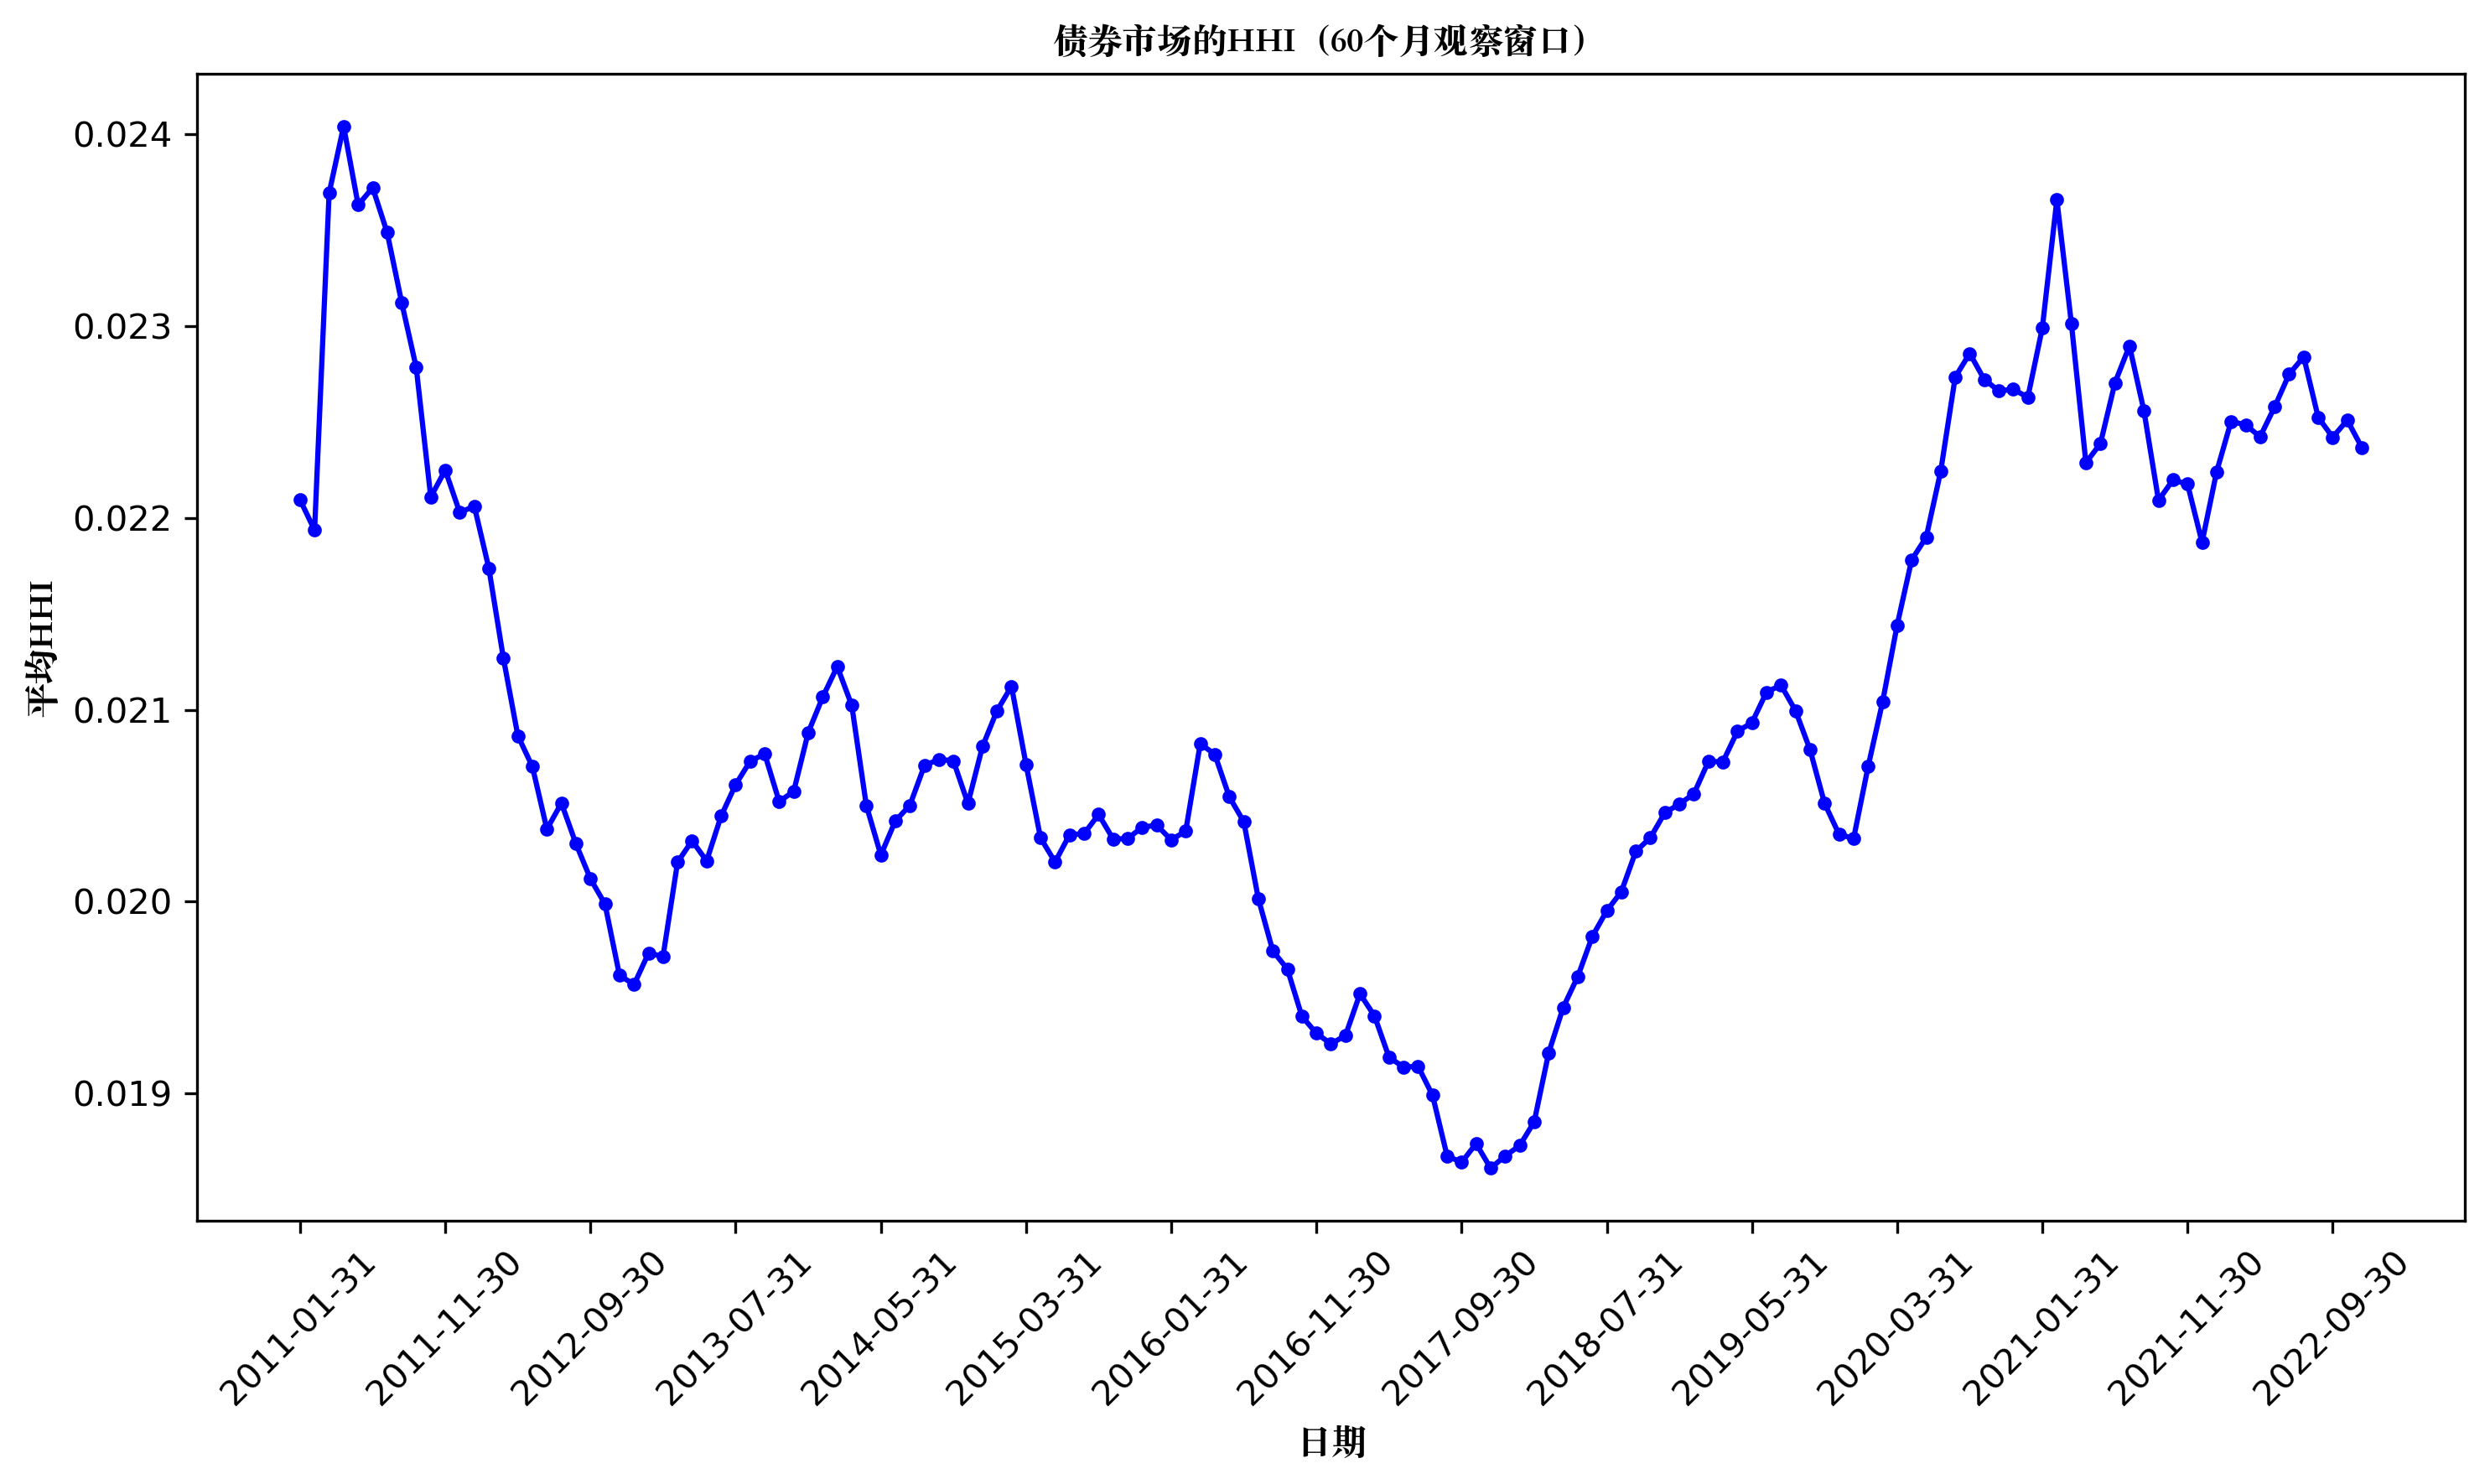
\includegraphics[scale=0.6]{figure/output1}
        \caption{市场层面的HHI时间序列线图}
        \label{fig:output1}
    \end{figure}
    观察时序图我们可以发现,从整个非银企业债券市场层面上来讲:债券到期的分散程度随着时间的变化没有明显的趋势;
    整体的债券到期HHI指标集中在0.019-0.024之间,远低于0.2。
    
    也就是说,整个非银企业的债券市场中债券到期的分散程度较高,期限结构较为合理。

    \section{企业层面的HHI}
    60个月度时间窗口的企业层面的HHI时间序列图如图\ref{fig:output2}所示。
    \begin{figure}[htbp]
        \centering
        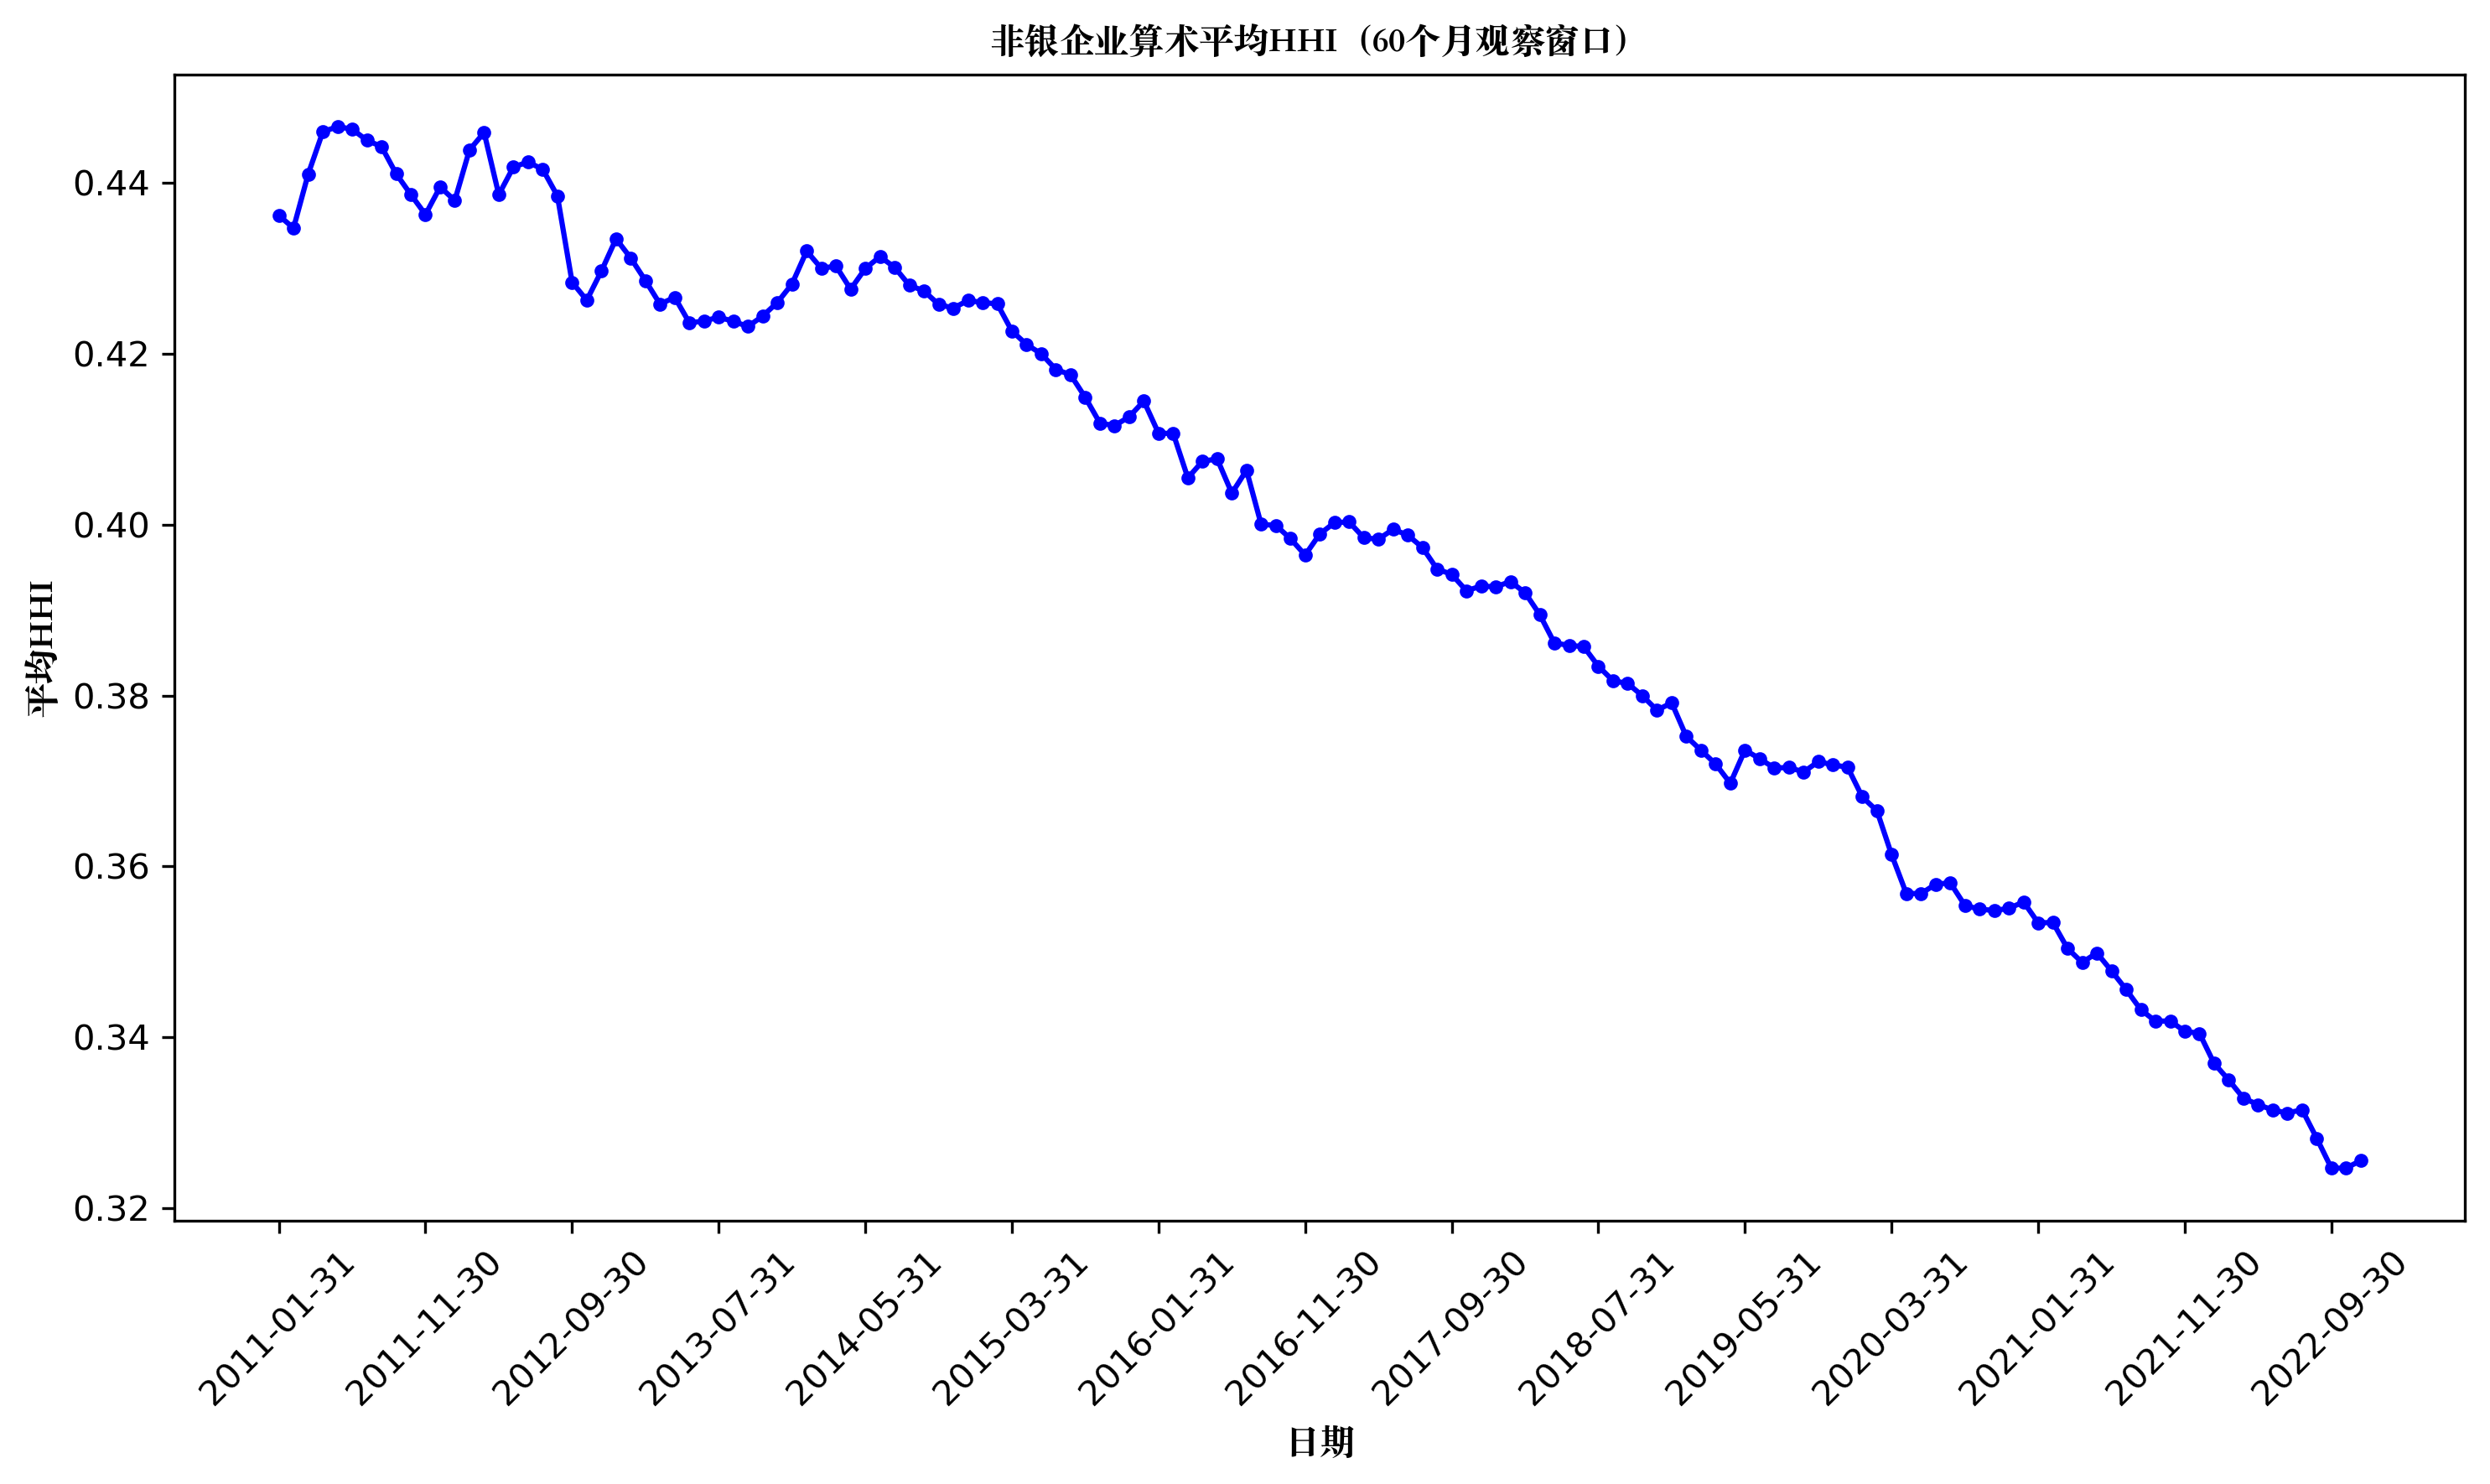
\includegraphics[scale=0.6]{figure/output2}
        \caption{市场层面的HHI时间序列线图}
        \label{fig:output2}
    \end{figure}
    
    观察时序图我们可以发现,从企业层面来看:债券到期的分散程度随着时间的增加呈现较为稳定的降低趋势;企业的债券到期HHI指标
    集中在0.32-0.44之间,明显高于0.2,且远远高于整体市场的HHI。

    由此发现,企业层面的HHI仍然较高,单个企业的债券的期限结构不够合理,应当更加均匀的分布。而分散程度逐年下降,有可能是
    企业的债券期限结构逐步改善,也有可能是按照月度观察,很多新债券难以发到同一个月导致HHI逐渐变小。为了解释这个现象,我们放大
    了观察时间窗口的长度为10年,以年度为分割绘制HHI的时序图。

    结果如图\ref{fig:output4}所示。
    \begin{figure}[htbp]
        \centering
        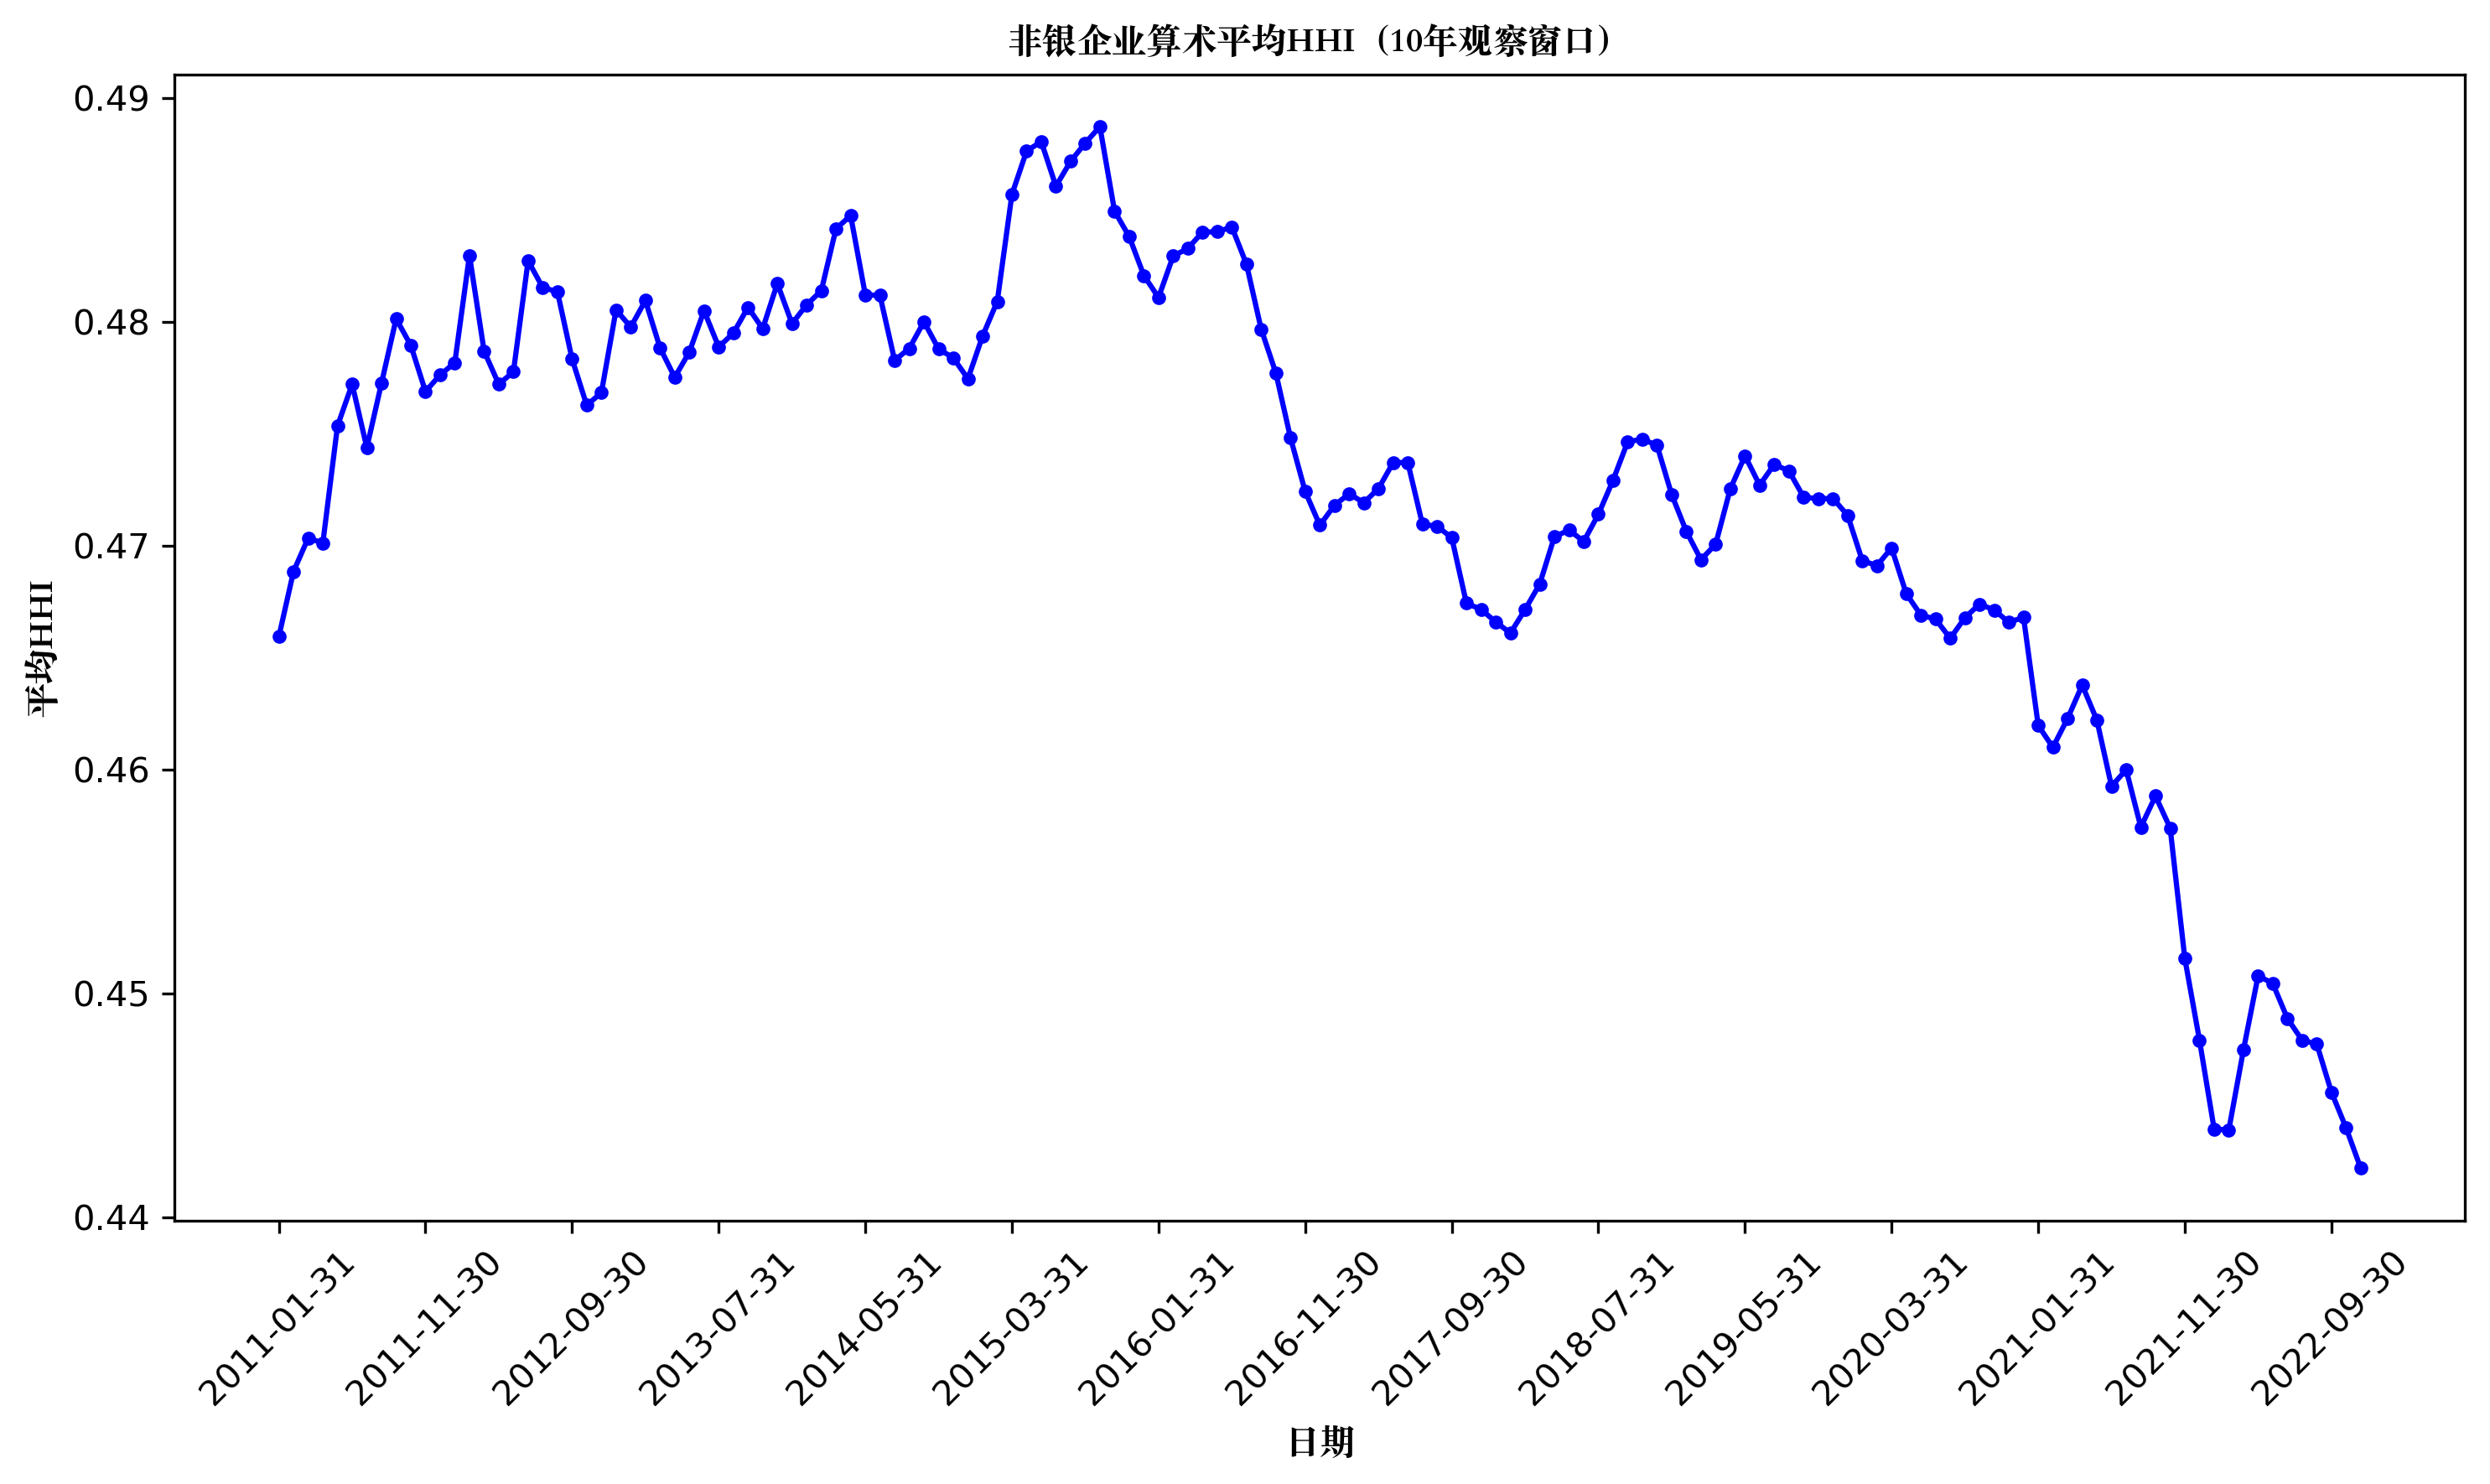
\includegraphics[scale=0.6]{figure/output4}
        \caption{市场层面的HHI时间序列线图}
        \label{fig:output4}
    \end{figure}

    观察图3发现,在此条件下,企业的债券到期HHI指标处于0.44-0.49之间,高于月度时间窗口的HHI值。因此,观察的时间窗口大小在一定程度上影响了
    企业的债券到期HHI指标。不过年度观察窗口下,HHI仍是波动降低的趋势,因此我们可以认为,中国非银企业的债券期限结构虽然当下仍然不够合理,
    但是呈现出了改善的趋势。
    

    \chapter{研究结论}
    本文基于中国非银企业的债券发行数据,通过构建不同观察时间窗口和不同观察视角的HHI时间序列来研究中国非银企业的债券期限结构是否合理。
    得出如下结论:

    1.中国的非银企业债券市场上的全部债券整体上期限是合理的,且不随着时间的变化有明显的变化。

    2.从企业层面来看,中国非银企业的债券期限结构当下仍然存在不合理的状态。

    3.随着时间的推移和市场的完善,企业层面上,债券期限结构在逐步地改善。
    %---------------------------------------------------------------------
    %  参考文献
    %---------------------------------------------------------------------

    \nocite{*}
    {\color{black} \printbibliography}

\end{document}


